\chapter{Jazyk Monkey C}
Monkey C \cite{monkeyc_2021} je objektově orientovaný jazyk navržený pro snadný vývoj Connect IQ aplikací. Jedná se o dynamický programovací jazyk, podobně jako Java, PHP či Ruby. Cílem Monkey C je zjednodušit proces vytváření samotné aplikace a umožnit tak vývojářům více se soustředit na zákazníka a méně na omezení zdrojů. Využívá tzv. "reference counting" k automatickému čištění paměti, což vývojáře osvobozuje od manuální správy paměti (např. jako v jazyce C/C++).
\\
\begin{figure}
	\centering
	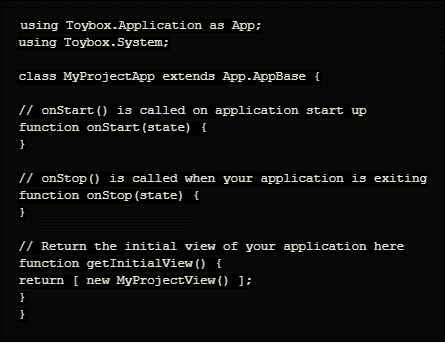
\includegraphics{images/code_snippet}
	\\
	\caption{ukázka jednoduchého fragmentu kódu v MonkeyC}
	\label{img:monkeyC_Fragment}
\end{figure}

\endinput